\chapter{Reimplementation of IPM in Ltac2}
\label{chap:reimplementation_ipm}

In the previous two chapters we covered both basics of separation logic and one of the tactic languages of Coq -- Ltac2.
This chapter is, to some extent, combining these two parts: we explain details of the implementation of Iris Proof Mode in Coq.

The original implementation of Iris Proof Mode is due to
\citet{krebbersInteractiveProofsHigherorder2017}.
It was later extended to MoSeL by \citet{krebbersMoSeLGeneralExtensible2018}, a general framework for modal separation logics in Coq.
This thesis builds on MoSeL and follows both its ideas and implementation closely.
However, while the original work was done using Ltac1, here we present a translation to Ltac2.

MoSeL itself, as evident from the title of the original paper, is a framework for separtion logic in Coq, which allows for easier formally verified proofs.
The idea is to embed separation logic in Coq and provide necessary infrastructure for a user to apply their intuitions and skills with tactics.

The structure of the chapter is as follows:
\begin{itemize}
\item First we describe the embedding of logic in Coq and how MoSeL entailments correspond to the theory.
\item Then we go into the details of the implementation of tactics and proof mode.
\item Finally, we share some experiences from the translation of Ltac1 implementation to Ltac2.
\end{itemize}

\section{MoSeL from theoretical perspective}
\label{sec:ipm_theory}
There are several options for embedding one (object) logic into another (meta) logic, but among them two most commonly used ones are ``shallow embedding'' and ``deep embedding''.

The first one corresponds to mapping propositions in the object logic directly to their semantics in meta-logic.
I.e.\ for classical separation logic we would map propositions to predicates over heaps.
This would map separating conjunction \(P * Q\) to \(\lambda \sigma.\,\exists\sigma_1, \sigma_2.\, \left(\sigma = \sigma_1 \uplus \sigma_2\right) \wedge P (\sigma_1) \wedge Q(\sigma_2)\) and separation logic entailment \(P \vdash Q\) to \(\forall \sigma. P \sigma \implies Q \sigma\).
Deep embedding, on the other hand, defines syntax of the object logic in meta-logic explicitly.

And while shallow embedding allows us to re-use meta-logic connectives and binders for some constructions, like implication in the example above, for others we have to make up more involved propositions.
This complicates proofs of entailments in the object logic when done within meta-logic.

Instead, MoSeL opts for abstraction of inference rules of the separation logic.
From a user perspective, this gives them both connectives and their inference rules, as well as some properties.
For separating conjunction user gets the usual commutativity, associativity and distributivity properties, as well as what MoSeL calls \textsc{sep-mono} rule:
\[(P_1 \vdash Q_1) \text{ and } (P_2 \vdash Q_2) \,\, \implies \,\, P_1 * P_2 \vdash Q_1 * Q_2\]
where ``and'' on the left-hand side and top-most implication are in the meta-logic.

However, while this allows axiomatic reasoning in object-logic, it still doesn't support tactics, which Coq users are used to.
For example, take the following entailment in affine separation logic:
\(P * Q * R \vdash R\).
A user would want to simply apply an ``assumption'' tactic (which we will use as a running example in this chapter), since relevant resource is clearly in the context and the rest can be discarded, using the following rule:

\[ \infer[\textsc{affine}]{P \vdash \emp}{\text{for any } P } \]

But without tactics this becomes cumbersome.
One solution would be convert right side of the entailment to \(\emp * (\emp * R)\) via double application of the property of \emp being neutral element for separating conjunction.
Then use \textsc{sep-mono} rule twice and ``drop'' both \(P\) and \(Q\) on the respective branches of the proofs using \textsc{affine} rule.

Naive implementation of tactics, however, would meet a problem: Coq tactics have an advantage of working in a structured context, instead of having an arbitrary bunch on the left-hand side of the entailment.
\citet{krebbersInteractiveProofsHigherorder2017} chose to restrict the context and instead of using arbitrary bunch, they propose a new entailment predicate:

\[\entailsOneD Q \defeq \Sep \Pi \vdash Q\]
where \(\SpatD\) is a list of pairs of identifiers and separation logic propositions \(\SpatD \defeq \left[H_1 : P_1, \ldots , H_n : P_n \right]\) and \(\Sep\) is an iterated separating conjunction.

If we substitute the definition of \(\SpatD\) and \(\Sep\), the entailment takes the following form:
\[\left( \entailsOne {H_1 : P_1, \ldots , H_n : P_n} Q \right) \defeq
  \left( P_1 * \ldots P_n \vdash Q \right)\]

In fact, the definition is slightly more general, as it incorporates two contexts: \(\IntuD\) and \(\SpatD\)
\[\entailsD Q\]
Where \(\IntuD\) is also a list of resources, but in the definition of the entailment it gets mapped to iterated non-separating conjunction with intuitionistic modality \(\intuit\):

\[\entailsD Q \defeq \intuit \left(\bigwedge \IntuD\right) * \left(\Sep \SpatD\right) \vdash Q\]

This allows easier introduction of new derivation rules, that are much closer to Coq tactics.

\subsection{Rules for regular IPM}
\label{sec:rules-regular-ipm}

Now that we have formalized Iris Proof Mode entailment, we can also render some tactics as derivation rules, instead of just Coq proof state transformers.
We aren't going to give a complete list of tactics, but just a few to illustrate the translation.

Regular introduction rules don't change that much, except now the context has to stay in a particular shape.

\begin{itemize}
\item To introduce a magic wand we extend the spatial context with a new resource.
  \[\infer[\textsc{Tac-wand-intro}]
      {\entailsD P \wand Q}
      {\entails {\IntuD} {\SpatD, i : P} {Q} &
       i \text{ is a fresh identifier}}
  \]
  If the resource introduced is intuitionistic, we can put it directly into an intuitionistic context, while stripping away the modality.
  \[\infer[\textsc{Tac-wand-intro-intuit}]
      {\entailsD \intuit P \wand Q}
      {\entails {\IntuD, i : P} {\SpatD} {Q} &
       i \text{ is a fresh identifier}}
  \]
\item The rule for separating conjunction also stays very similar to the original one
  \[\infer[\textsc{Tac-sep-intro}]
      {\entailsD P * Q}
      {\entails {\IntuD} {\SpatD_1} P &
       \entails {\IntuD} {\SpatD_2} Q &
       \SpatD \equiv \SpatD_1 {+\hspace{-0.5em}+} \SpatD_2}
   \]
   \todo{swap for real append operator}
   Where \({+\hspace{-0.5em}+}\) is \coqe{append} operator for lists and \(\equiv\) is list equivalence modulo permutations.

   Note that intuitionistic context doesn't have to be split, since resources in it are duplicable, hence we can access them in both branches of the proof.
\item Before we get to \coqe{assumption} tactic, let's consider \coqe{exact H}, which closes goals with assumption \coqe{H} from the context.
  The following would be a correct, but not very useful tactic:
  \begin{align*}
      \infer
        {\entailsD P}
        {\SpatD = [H : P]}
    & \hspace{5em}
    & \infer
        {\entails {\IntuD} {[\,]} P}
        {H : P \in \IntuD}
  \end{align*}
  In the first case here there aren't any requirements for the intuitionistic context, since resources in it are affine by definition.
  This doesn't hold for spatial context in general unless the logic we're working is affine.

  However, both of the variants put significant restrictions on spatial context, which can be lifted slightly.
  As noted above, one could create a specialized tactic for affine logic, but instead MoSeL asks for the rest of the context to only contain affine resources, so the tactic becomes:
  \begin{align*}
      \infer%[\textsc{tac-exact-spatial}]
        {\entailsD P}
        {H : P \in \SpatD &
         \SpatD \backslash (H : P) \text{ is affine}}
    & \hspace{5em}
    & \infer%[\textsc{tac-exact-intuitionistic}]
        {\entails {\IntuD} {[\,]} P}
        {H : P \in \IntuD &
         \SpatD \text{ is affine}}
  \end{align*}
  We call a context affine if it only contains affine resources and stick to convention that in affine logic all resources are affine.
\item Generalization of the tactic above to behave more like \coqe{assumption} is trivial -- instead of asking for a specific \(H : P\) to be in the context, we ignore identifiers entirely and the assumption becomes that there is some \(P\) in the context
  \begin{align*}
      \infer%[\textsc{tac-assumption-spatial}]
        {\entailsD P}
        {\exists H. H : P \in \SpatD &
         \SpatD \backslash (H : P) \text{ is affine}}
    & \hspace{5em}
    & \infer%[\textsc{tac-assumption-spatial}]
        {\entailsD P}
        {P \in \IntuD &
         \SpatD \text{ is affine}}
  \end{align*}
\end{itemize}

% \begin{itemize}
% \item Start proof
% \item Context maninputation
%   \begin{itemize}
%   \item iRename
%   \item iClear
%   \item iEval
%   \end{itemize}
% \item Assumptions
%   \begin{itemize}
%   \item iExact
%   \item iAssumption
%   \end{itemize}
% \item Intuitionistic/Spatail/Pure transitions
%   \begin{itemize}
%   \item iIntuitionistic
%   \item iSpatial
%   \item iPure
%   \item iEmpIntro
%   \item iPureIntro
%   \end{itemize}
% \item iFrame
% \item Intro of wand/implication
% \item Revert
% \item Specialize and Pose
% \item Apply
% \item Existential
%   \begin{itemize}
%   \item Intro
%   \item Destruct
%   \end{itemize}
% \item Modalities
% \item iDestruct
% \item iIntros
% \item Induction
% \item Löb
% \item Assert
% \item Rewrite
% \end{itemize}

\subsection{Implementation of IPM}
\label{sec:implementation-of-ipm}

Now that we have seen Iris Proof Mode from theoretical perspective, let's turn to Coq implementation.

We start with an overview of components of the implementation and build \coqe{iAssumption} tactic in the end.

\begin{figure}[H]
  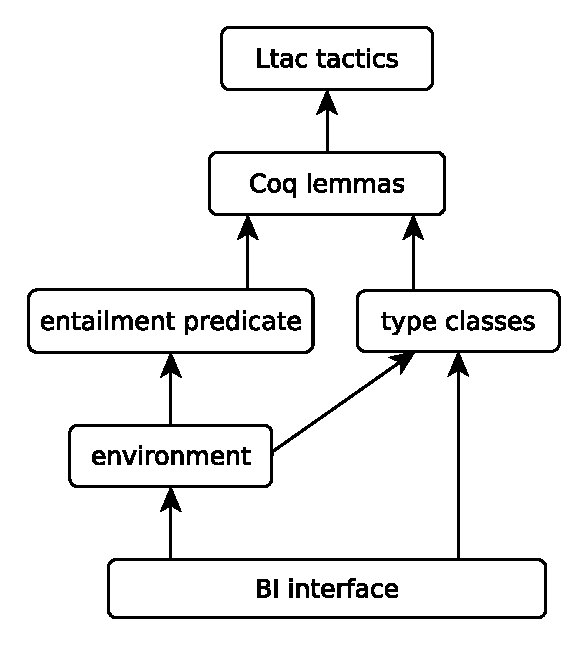
\includegraphics[width=0.5\linewidth]{ipm-diagram}
  \caption{structure of the implementation of IPM}
  \label{fig:ipm-diagram}
\end{figure}


\begin{itemize}
\item The base layer of the implementation is a BI interface, which user instantiates with their logic and can profit from the existing infrastructure.
\item On top of the BI interface MoSeL defines environments and entailment predicates. These are used to make proofs of ``Coq tactics'' easier and typeclasses allow for more general unification and proof search.
\item ``Coq tactics'' themselves are verified transformations of the goal, the simplest instance being \coqe{tac_ex_falso}, which looks as follows:\\
\coqe{Lemma tac_ex_falso Delta Q : envs_entails Delta False → envs_entails Delta Q.}.
\item These transformations are then applied by Ltac2 programs, which can combine them, use specialized tactics for the subgoals they generate and handle errors.
\end{itemize}


\subsubsection{BI interface}
\label{subsubsec:bi-interface}

There are five main components, starting with a base interface for BI logic, which we mentioned before and which \citet{krebbersMoSeLGeneralExtensible2018} call MoBI interfaces, for Modal BI.

We include it here, with some omissions:
\begin{coq}
Structure bi := Bi {
  bi_car :> Type;
  bi_dist : Dist bi_car;
  bi_emp : bi_car;
  bi_and : bi_car → bi_car → bi_car;
  bi_forall : forall A, (A → bi_car) → bi_car;
  bi_sep : bi_car → bi_car → bi_car;
  bi_wand : bi_car → bi_car → bi_car;
  bi_persistently : bi_car → bi_car;
  bi_pure : Prop → bi_car;
  bi_bi_mixin : BiMixin $\ldots$;
  $\ldots$
}.
\end{coq}

Where \coqe{BiMixin} is a field that describes axioms that connectives should satisfy, from associativity of separating conjunction to elimination rule for persistent modality.
With some notation definitons this allows writing and proving BI propositions, only requiring an instance of \coqe{bi}.

\begin{minipage}{\linewidth}
\begin{coq}
Context {PROP : bi}.
Lemma persistently_mono P Q : (P |- Q) → <pers> P |- <pers> Q.
\end{coq}
\end{minipage}

Proving such statement, however, at this point still requires applying axioms from \coqe{bi} by hand.

\subsubsection{Environments and entailment predicate}
\label{subsubsec:environment-entailment-pred}

In order to define IPM entailment, we first define contexts.
In general, since most of the tactics only have to deal with one hypothesis from the context or don't even touch existing ones (like \coqe{iIntro}), \citet{krebbersMoSeLGeneralExtensible2018} use deep embedding to allow easier syntactical transformations.

Environments are defined as association lists with identifiers used as keys and BI propositions as values.

\begin{coq}
Inductive ident :=
  | IAnon : positive -> ident
  | INamed :> string -> ident
Inductive env (A : Type) : Type :=
  | Enil : env A
  | Esnoc : env A -> ident -> A -> env A.
\end{coq}

However, as described above MoSeL entailment predicate includes two context: spatial and intuitionistic, so we have to define another structure to include both:

\begin{coq}
Record envs (PROP : bi) := Envs {
  env_intuitionistic : env PROP;
  env_spatial : env PROP;
  env_counter : positive (** A counter to generate fresh hypothesis names *)
}.
\end{coq}

Then we can define entailment predicate, which includes not only both contexts, but also a proof that identifiers in each context are unique \coqe{envs_wf $\Delta \urcorner$}.
\begin{coq}
  Definition envs_entails {PROP} ($\Delta$ : envs PROP) (Q : PROP):
  $\ulcorner$ envs_wf $\Delta \urcorner$ /\ $\intuit$ [$\wedge$] env_intuitionistic $\Delta$ * [*] env_spatial $\Delta$ |- Q
\end{coq}

Here \coqe{[*]} is an iterated separating conjunction, defined on lists as folds with respective operation, the same way as it was defined in theoretical presentation.

At this point we can already make some statements in both readable and easy to prove form, such as \coqe{tac_ex_falso}, which we mentioned before.\\
\coqe{Lemma tac_ex_falso Delta Q : envs_entails Delta False → envs_entails Delta Q.}

\subsubsection{Typeclasses}
\label{subsubsec:typeclasses}

Typeclasses serve multiple purposes in MoSeL development, here we are going to describe only couple of simplest instances needed for \coqe{iAssumption}.
The primary idea is to automatize simple parts of proof search via logic programming.

The first example we are going to look at are \coqe{Affine} and \coqe{AffineEnv}.
The former is defined simply as
\begin{coq}
Class Affine {PROP : bi} (Q : PROP) := affine : Q |- emp.
\end{coq}

With instances covering both basic connectives
\begin{coq}
Global Instance emp_affine : Affine emp.
Global Instance and_affine_l P Q : Affine P → Affine (P /\ Q).
Global Instance and_affine_r P Q : Affine Q → Affine (P /\ Q).
Global Instance sep_affine P Q : Affine P → Affine Q → Affine (P * Q).
$\ldots$
\end{coq}

And modalities
\begin{coq}
Global Instance affinely_affine P : Affine (<affine> P).
Global Instance affinely_if_affine p P : Affine P → Affine (<affine>?p P).
Global Instance intuitionistically_if_affine p P : Affine P → Affine ($\intuit$?p P).
\end{coq}
Conditional modalities, like \coqe{<affine>?p P} are defined as \coqe{(if p then <affine> P else P)}.


For the environment to be affine we simply require all resources in the context to be affine and declare instances for both constructors.
\begin{coq}
Class AffineEnv (Γ : env PROP) := affine_env : Forall Affine Γ.
Global Instance affine_env_nil : AffineEnv Enil.
Global Instance affine_env_snoc Γ i P :
  Affine P → AffineEnv Γ → AffineEnv (Esnoc Γ i P).
\end{coq}

The next example is slightly more involved and concerns entailment of one proposition with another.
To be more precise, we want to define a typeclass which corresponds to intuitive ``\(P\) is almost the same as \(Q\) and P entails Q''.
\begin{coq}
Class FromAssumption {PROP : bi} (p : bool) (P Q : PROP) :=
  from_assumption : $\intuit$?p P |- Q.
\end{coq}

There are two subclasses of it, providing instances where either the first or the second proposition is treated as an input.
\begin{coq}
Class KnownLFromAssumption {PROP : bi} (p : bool) (P Q : PROP) :=
  knownl_from_assumption :> FromAssumption p P Q.
Class KnownRFromAssumption {PROP : bi} (p : bool) (P Q : PROP) :=
  knownr_from_assumption :> FromAssumption p P Q.
\end{coq}

The difference between their instances is that for \coqe{KnownLFromAssumption} we ``match'' input \(P\) with structural rules and Q is an output and vice-versa for \coqe{KnownRFromAssumption}.
This allows for more effective search, but for our purposes it is a mere technicality, so we will only consider \coqe{KnownRFromAssumption}.

\begin{coq}
Lemma from_assumption_exact {PROP : bi} p (P : PROP) : FromAssumption p P P.
\end{coq}

While the simplest instance of this is just an identity \coqe{P |- P}, there are several more defined in MoSeL, which generalize it.
For example, given that we can prove \(\intuit P \vdash Q\), we can also prove \(\intuit P \vdash \affine Q\) and  \(\intuit P \vdash \intuit Q\).
\begin{coq}
Global Instance from_assumption_affinely_r P Q :
  FromAssumption true P Q → KnownRFromAssumption true P ($\affine$ Q).
Global Instance from_assumption_intuitionistically_r P Q :
  FromAssumption true P Q → KnownRFromAssumption true P ($\intuit$ Q).
\end{coq}

\subsubsection{Coq tactics}
\label{sec:coq-tactics}

As mentioned above, Coq tactics are verified goal transformations, which can be as simple as rules for \coqe{exfalso}, but also more advanced, like the one for \coqe{assumption}.

The idea is that we are provided an identifier of the resource that is in the context and should check all side conditions: the resource is indeed there, it coincides with the goal and other resources can be safely discarded.

\begin{figure}[H]
\begin{coq}
Lemma tac_assumption Delta i p P Q :
  envs_lookup i Delta = Some (p,P) →
  FromAssumption p P Q →
  (let Delta' := envs_delete true i p Delta in
   if env_spatial_is_nil Delta' then TCTrue
   else TCOr (Absorbing Q) (AffineEnv (env_spatial Delta'))) →
  envs_entails Delta Q.
\end{coq}  
\caption{\coqe{tac_assumption} definition}
\label{fig:tac-assumption}
\end{figure}

\coqe{envs_lookup} returns a boolean for the context it found identifier \coqe{i} within and proposition \(P\) that was associated with it.

Second assumption guarantees that \(P\) entails \(Q\) and the last one checks that we can discard the rest of the spatial resrouces in \(\Delta\).
If spatial context is empty, there is nothing to discard, but otherwise either the whole environment must be affine, or the goal should be able to absorb them:
\(\Absorbing Q \defeq \forall Q, P * Q \vdash \absorb P\).

No other subgoals are generated, since this is a leaf of a derivation.

\subsubsection{Ltac2 tactics}
\label{sec:ltac2-tactics}

The final piece of the puzzle is Ltac2 layer.
While Coq tactics provide verified goal transformations, they require several inputs.
The balance between what should go into a Coq statement and Ltac2 function is about how easy is it to verify something.

Turning again to \coqe{iAssumption}, the idea is that a user doesn't provide explicit identifier of the resource they have in mind, instead tactic is supposed to find it on its own.

Simply asserting existence of such identifier in a Coq lemma doesn't solve anything, since ultimately we have to apply this transformation to the goal and user will have to provide it, hence universally quantified identifier in the definition of the Coq lemma \ref{fig:tac-assumption}.

Instead, we go through all elements of the environment in Ltac2 and try to apply the lemma with each one.

\begin{figure}
\begin{coq}
Ltac2 i_assumption () :=
  let rec find (p : coq_bool) (g : ipm_env) (q : ipm_prop) :=
      lazy_match! g with
      | Esnoc ?gg ?j ?pp =>
        first [ refine '(tac_assumption _ \$j \$p \$pp _ _ _ _) >
                [ pm_reflexivity () (* for the lookup *)
                | i_solve_tc () (* perform typeclass search for FromAssumption*)
                | pm_reduce (); (* evaluate env_delete and if-branch *)
                  i_solve_tc ()]
              | find p gg q]
      end
  in
  lazy_match! goal with
  | [|- envs_entails (Envs ?gp ?gs _) ?q] =>
     first [ find '(true) gp q
           | find '(false) gs q
           | i_assumption_coq ()
           | Control.zero (Iriception (of_string "no assumption matching " ++
                                       of_constr q ++
                                       of_string " was found"))]
  end.
\end{coq}  
\caption{\coqe{i_assumption} definition}
\label{fig:i-assumption-def}
\end{figure}

The listing is in Figure \ref{fig:i-assumption-def}.
Since there are two contexts to go through, we factor out recursion into a \coqe{find} function, which takes a Boolean flag \coqe{p} to tell apart spatial and intuitionistic context, context \coqe{g} and proposition \coqe{q}.
Then we apply \coqe{tac_assumption} defined above~\ref{fig:tac-assumption} and discharge the goals with specialized tactics.
The first subgoal \coqe{envs_lookup i Delta = Some (p,P)} is computational, so \coqe{pm_reflexivity ()} performs evaluation and tries \coqe{reflexivity} tactic.
The other two concern type classes, so we use a wrapper around \coqe{typeclasses eauto} to solve them.

The only part which wasn't described so far is \coqe{i_assumption_coq ()}.
This is an example of tactics composition -- \coqe{i_assumption_coq} is essentially applying a different lemma from \coqe{tac_assumption}, which tries to find an assumption of shape \(\vdash Q\) in the Coq context instead of IPM context.

This example also showcases some error handling in the last case, if none of the cases listed before it succeed.

\section{Improvements from translation to Ltac2}

While translating implementation from Ltac1 to Ltac2, we encountered several points where Ltac2 was particularly useful.

\paragraph{Fix arities from original IPM}

In the original implementation there aren't tactics of arbitrary arity.
Instead, due to Ltac limitations, developers were forced to define several variants of tactics, each with fixed arity.

\begin{coq}
Tactic Notation "iExists" uconstr(x1) "," uconstr(x2) :=
  iExists x1; iExists x2.
Tactic Notation "iExists" uconstr(x1) "," uconstr(x2) "," uconstr(x3) :=
  iExists x1; iExists x2, x3.
Tactic Notation "iExists" uconstr(x1) "," uconstr(x2) "," uconstr(x3) ","
    uconstr(x4) :=
  iExists x1; iExists x2, x3, x4.
\end{coq}

With Ltac2 we can use scopes for lists, which allow arbitrary arities.
The example above would look as follows:

\begin{coq}
  Ltac2 Notation "iExists" lc(list1(thunk(seq(constr, with_bindings)), ",")) :=
  i_exists lc.
\end{coq}

Where \coqe{i_exists} iterates over the list and applies \coqe{iExists} to each element.

\paragraph{Error messages}

Another pain point of Ltac development is lack of proper error handling.

With Ltac2 there two features that help -- we can define our own custom error classes and there is a proper error handling mechanism, which allows us to match on the error thrown.

As with the \coqe{i_assumption} above, there are multiple instances of nesting tactics within each other.
One way to improve error message thrown by iAssumption would be to catch potential error thrown by \coqe{i_assumption_coq} and append it to the error message produced in \coqe{i_assumption}, so that user can see why the tactic failed.

\section{Desirable features in Ltac2}

However, there also were several features that we wished Ltac2 had and that impacted the scope of potential improvements.

\paragraph{User-defined scopes}

Perhaps, one of the useful features of the original IPM implementation that is missing from our implementation is intropatterns.
The proper way to define them with Ltac2 would be to extend datatype for intropattern with IPM-specific symbols and then parse it with a custom scope.

Unfortunately, the latter isn't currently possible without extending OCaml implementation of Ltac2, either via forking Coq or using an Ocaml plugin that modifies Ltac2 grammar.

\paragraph{User-defined pretty-printing}
Another missing feature would be lack of user-defined printing rules.
At the moment this mostly impacts error printing, since we have to rely on the Ltac2 pretty-printer, as notations are parsing-only.

\paragraph{notypeclasses refine}

Ltac2 also currently lacks a variant of \coqe{refine}, which doesn't resolve typeclasses on the application.
This tactic is heavily used in MoSeL development.

\paragraph{Interoperability between Ltac1 and Ltac2}

While the goal of the rewriting was to give platform for further experiments, some of the tactics were easier to import.
And while there is a way to call Ltac1 tactics from Ltac2 code, there is no proper way to pass return values there or back.
I.e.\ \href{https://gitlab.mpi-sws.org/iris/string-ident/}{iris string-ident} has to pass terms through the goal to get the result from one to another.

%%% Local Variables:
%%% mode: latex
%%% TeX-master: "thesis"
%%% TeX-parse-self: t
%%% TeX-auto-save: t
%%% reftex-cite-format: natbib
%%% reftex-default-bibliography: ("/home/buzzer/my-dir/ed/uni/saar/prjcts/iris/npm/tex/TacticsProofs.bib")
%%% End: